\section{Research Methodology}
\label{sec:Res}
\par This section is one of the most important parts of your research and it is the one that will receive most criticism. The reason is that here you document how you conducted your research. Since you are reading a B.Sc. degree you are expected to follow a scientific method, thus in this section you are expected to document: \textbf{the problem}; \textbf{hypothesis}; \textbf{aim \& objectives}; \textbf{research questions}; and \textbf{research pipeline}. Let's go through each.

\par First start by providing a brief overview of the problem, similar to what you already mentioned in the previous sections. Then provide a hypothesis, this is the assumption you are making, which via your research you are attempting to prove or disprove. An example hypothesis in traffic management would be: \textit{By using image processing on public camera video feeds we believe that it is possible to estimate the traffic congestion at a higher precision than public traffic data feeds.}

\par After explaining the problem and hypothesis you need to specify why you are doing this research and what you think the output will be, so the aim \& objectives. Let us consider the \enquote{Marine Vessel Tracking} concept: \textit{With this research we aim to be able to automatically detect any anomalies within Marine traffic, such as drug smuggling, human trafficking and/or collisions.} Our objectives are:
\begin{enumerate}
    \item Identify existing data sets and manners of connecting them or even enriching them.
    \item Review existing algorithms and propose a suitable model
    \item Evaluate the effectiveness of the proposed model with real data and existing research.
\end{enumerate}

\par So lastly you have to present a number of research questions that you attempt to answer, which ideally revolve around the \textbf{data set}, \textbf{algorithm} and \textbf{evaluation} which you documented in your literature review:
\begin{enumerate}
    \item Does a data set need to be created for such a research?
    \item Which current technology is best suited to address the problem?
    \item How does the proposed solution compare with existing solutions?
\end{enumerate}

\par Finally, you need a plan on how you intend to answer the research questions which will help you prove/disprove the hypothesis. Different research areas would require specific pipelines, yet a generic one is shown in Fig~\ref{fig:Pipeline}. After presenting an illustration of your pipeline it is recommended to documenting what has been done at every stage. Remember you should use past tense in this section since you are document what you have already done, since this paper will be published at the end of your research.

\begin{figure}[ht]
    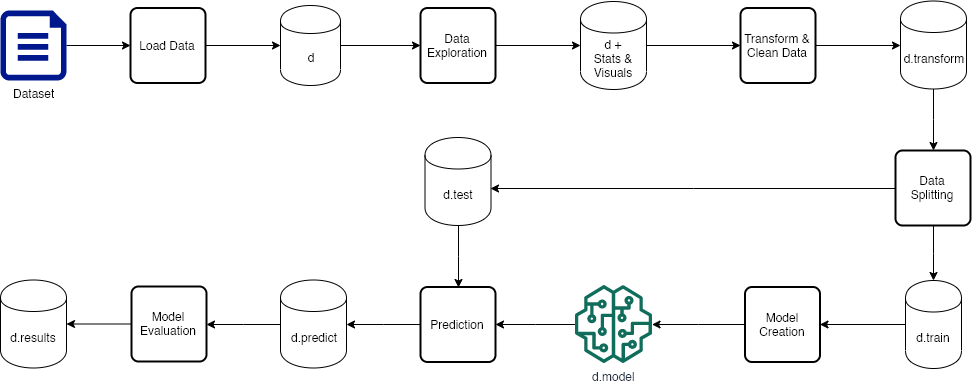
\includegraphics[scale=0.25]{includes/pipeline.png}
    \centering
    \caption{Research Pipeline}
    \label{fig:Pipeline}
\end{figure}